\section{Joint State Estimation (4.1)}

\subsection{Description of the algorithm}
We use the algorithm described under section 1.1 to estimate the
3D coordinates of each of the joints.
We use our \texttt{fit\_theta1} method to optimise the error of fitting
our angles to the estimated 3D coordinates:
\begin{enumerate}
    \item
        For various "guesses" in the range of $[-\pi, \pi]$, let
        $\hat{\theta_1}$ be a guess for the first joint.
    \item
        "Undo" this guess by rotating around the Z-axis by $-\hat{\theta_1}$
    \item
        Estimate the angles for $\theta_2, \theta_3, \theta_4$ using our
        previously described approach.
    \item
        Compute the positions of the \textbf{green} and \textbf{red}
        joint using forward kinematics, and \textbf{compute the error}
        between our 3D estimates and these locations.
    \item
        We let our estimate for $\theta_1$ be the angle which minimises
        the error described above.

\end{enumerate}

\subsection{Comparing estimations with sinusoidal signals} \label{4_1_sinus_plots}
\begin{tabular}{c c}
    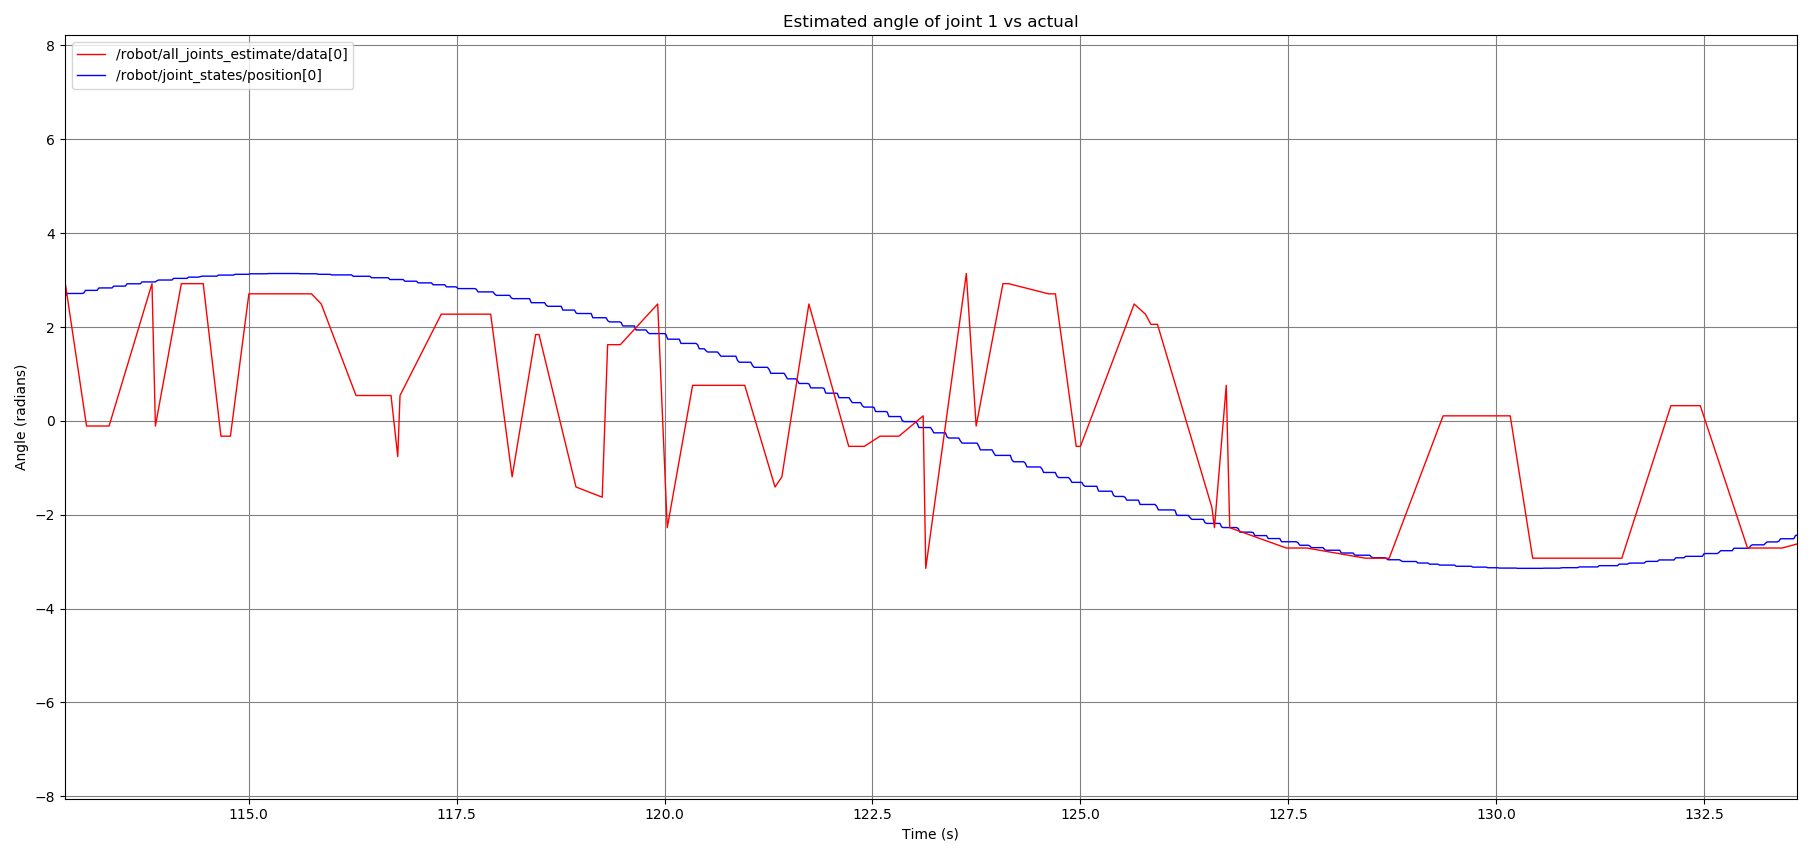
\includegraphics[width=0.5\linewidth]{plots/joint1_q4.png} &
    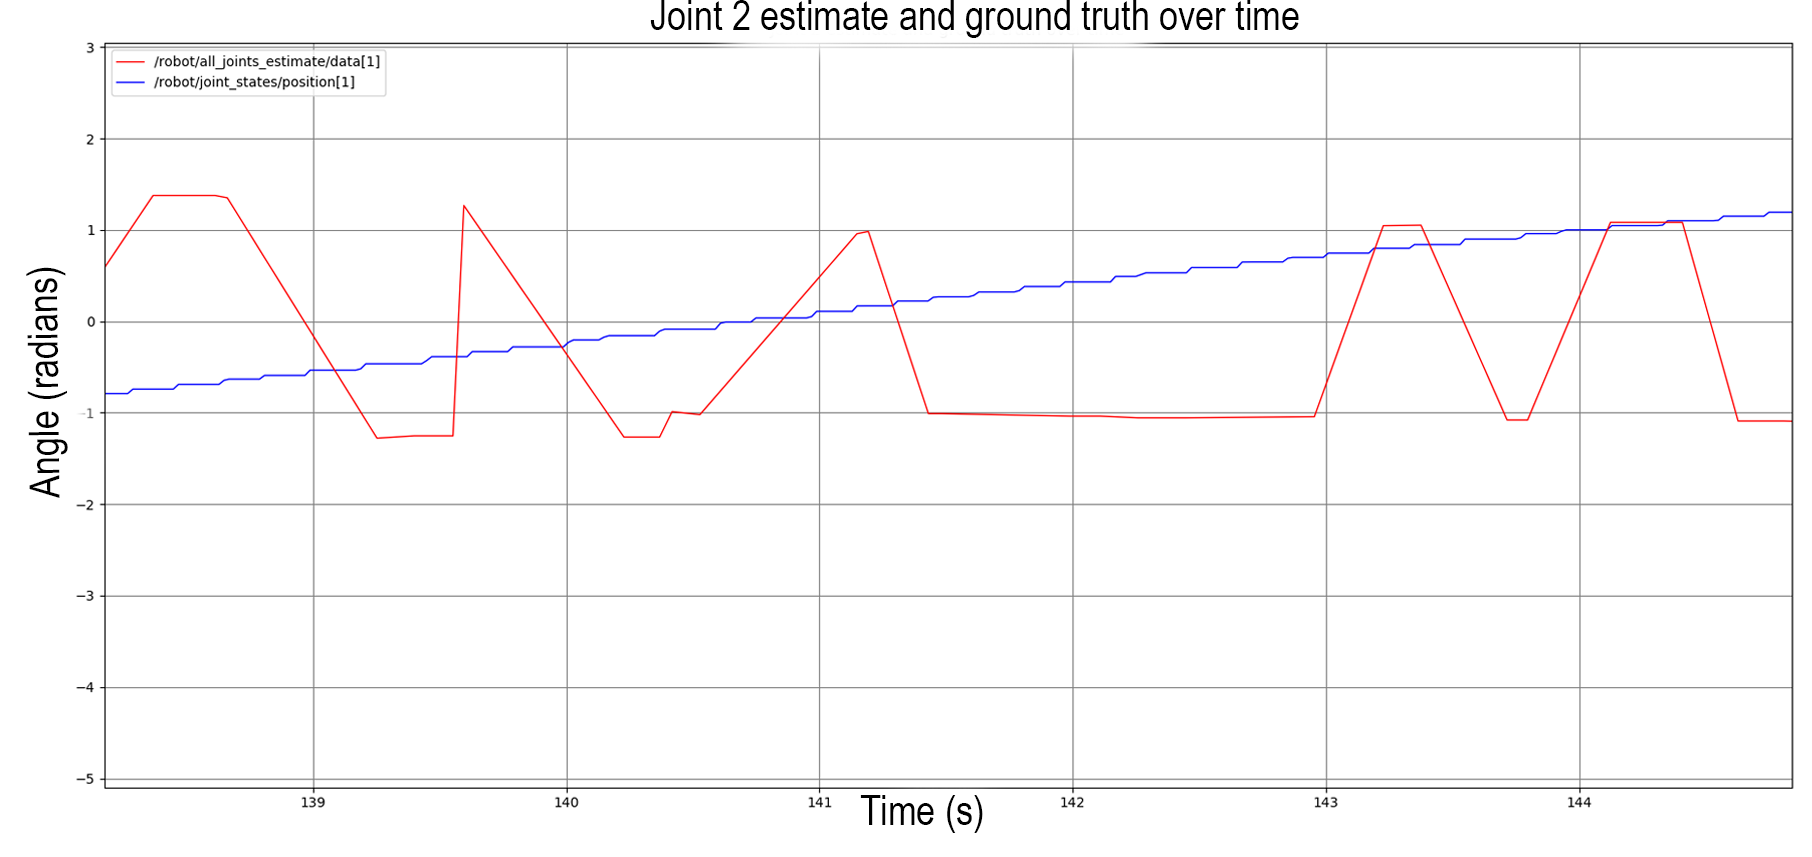
\includegraphics[width=0.5\linewidth]{plots/joint2_q4.png} \\
    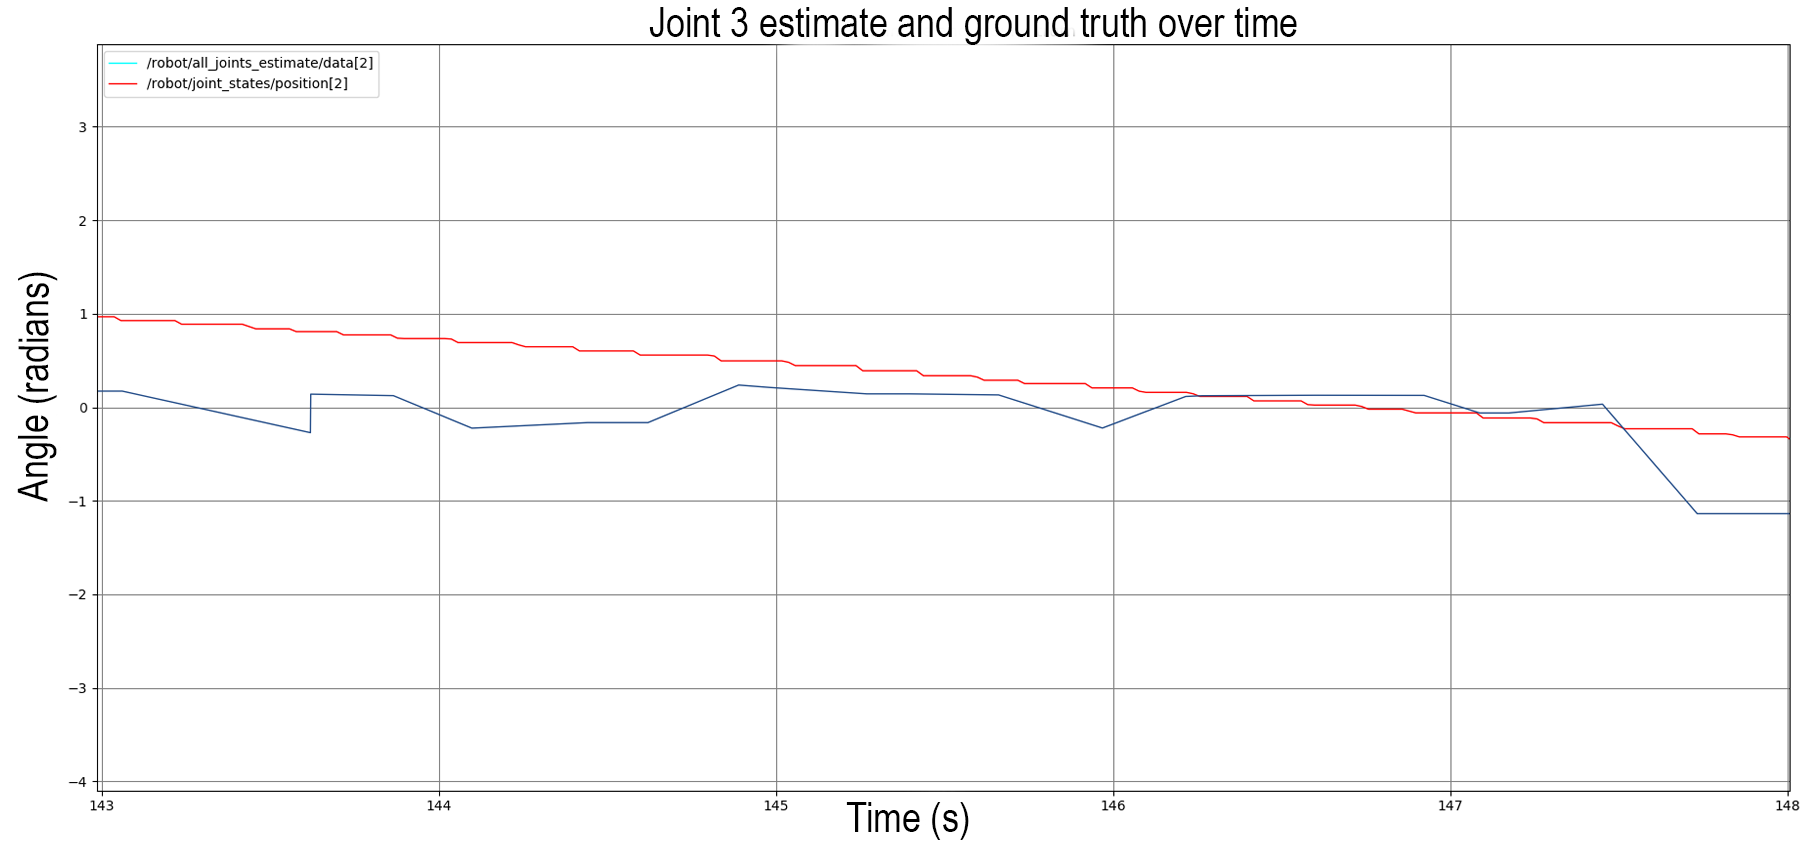
\includegraphics[width=0.5\linewidth]{plots/joint3_q4.png} &
    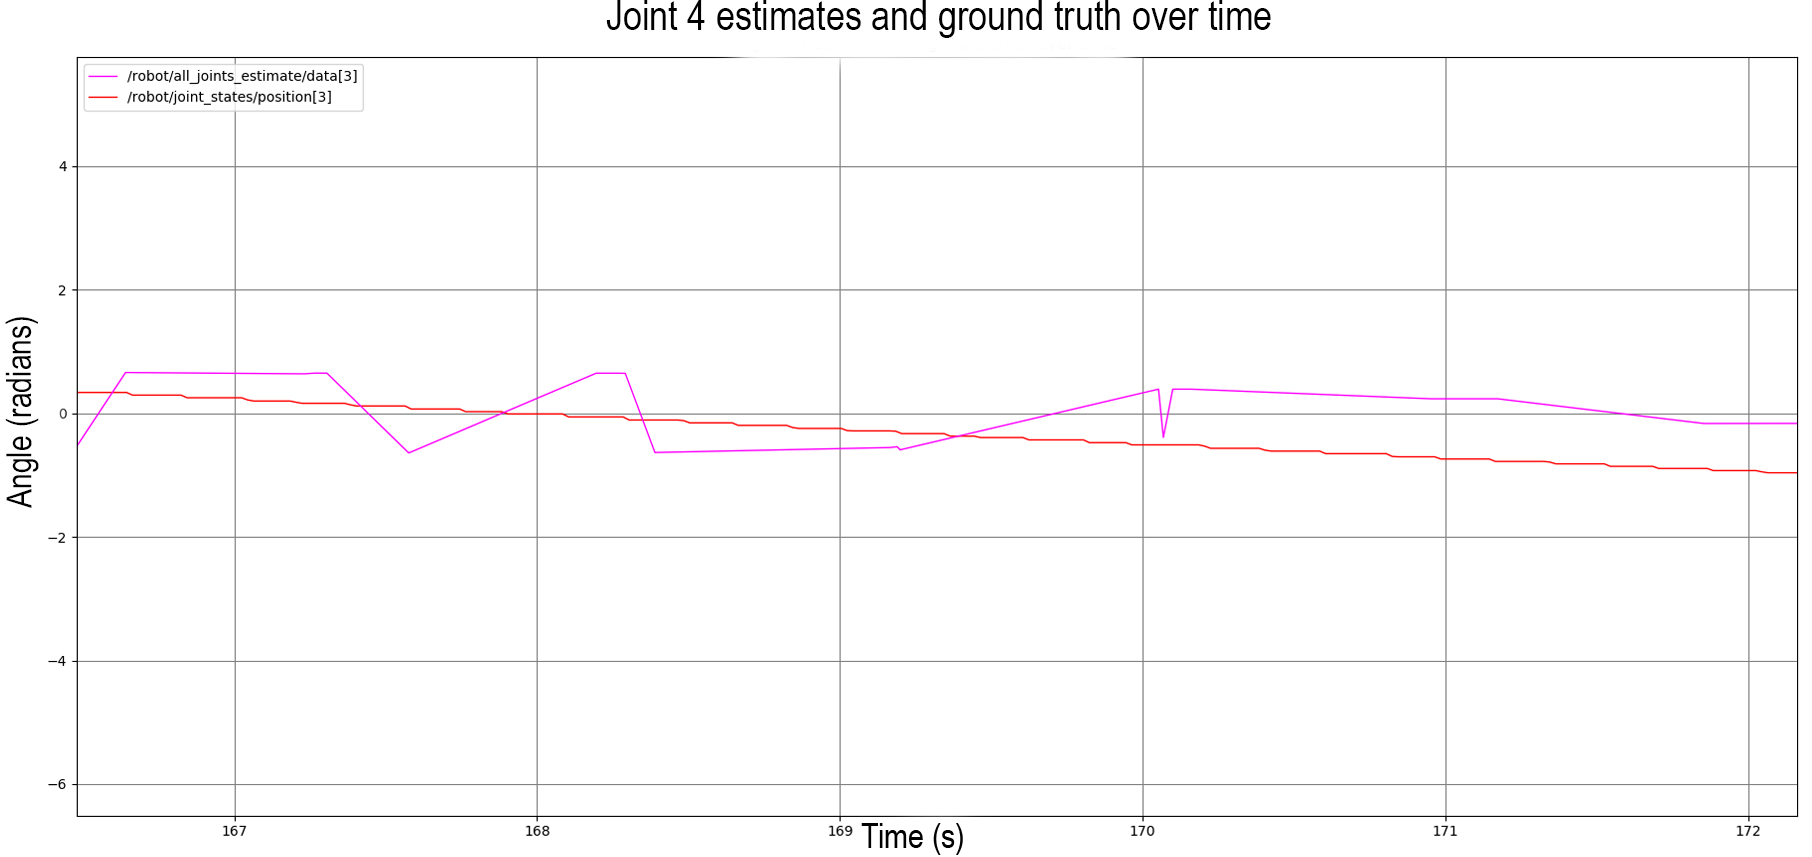
\includegraphics[width=0.5\linewidth]{plots/joint4_q4.png}
\end{tabular}

\subsubsection{Comparing joint1 estimates with ground truth}
Unfortunately, our 3D joint location estimates are not accurate enough
to estimate $\theta_1$ accurately.\\
In order to show that our approach does work given correct 3D estimates,
we decided to compare our estimate to ground truth:\\
Let robot state be $\text{R} = \begin{bmatrix}
    \theta_1 \\
    \frac{1}{6} \pi \\
    -\frac{1}{6} \pi \\
    -\frac{1}{4} \pi
\end{bmatrix} $. Let $\hat{\theta_1}$ be our estimate of $\theta_1$:
\begin{center}
    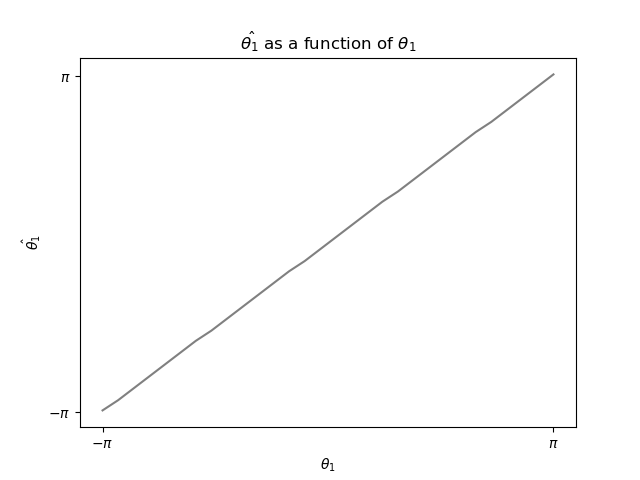
\includegraphics[width=0.4\linewidth]{plots/theta1_estimation.png}
\end{center}
Our algorithm is able to accurately estimate the value of $\theta_1$,
as long as we supply accurate 3D locations for each of the joints.
Therefore, we believe the inaccuracies in the plots in section~\ref{4_1_sinus_plots}
are caused by the inaccuracy stemming from our vision algorithm.
